\documentclass{article}


\usepackage{PRIMEarxiv}

\usepackage[utf8]{inputenc} % allow utf-8 input
\usepackage[T1]{fontenc}    % use 8-bit T1 fonts
\usepackage{hyperref}       % hyperlinks
\usepackage{url}            % simple URL typesetting
\usepackage{booktabs}       % professional-quality tables
\usepackage{amsfonts}       % blackboard math symbols
\usepackage{nicefrac}       % compact symbols for 1/2, etc.
\usepackage{microtype}      % microtypography
\usepackage{lipsum}
\usepackage{fancyhdr}       % header
\usepackage{graphicx}       % graphics
\usepackage{amsmath}
\usepackage{float}
\graphicspath{{media/}}     % organize your images and other figures under media/ folder

%Header
\pagestyle{fancy}
\thispagestyle{empty}
\rhead{ \textit{ }} 

% Update your Headers here
\fancyhead[LO]{Comparative Analysis of Diffusion Models for Image Generation}
% \fancyhead[RE]{Firstauthor and Secondauthor} % Firstauthor et al. if more than 2 - must use \documentclass[twoside]{article}



  
%% Title
\title{Comparative Analysis of Diffusion Models for Image Generation
%%%% Cite as
%%%% Update your official citation here when published 
%\thanks{\textit{\underline{Citation}}: 
%\textbf{V. Sharan. Comparative Analysis of Diffusion Models for Image Generation.}} 
}

\author{
  Vaibhav Sharan\\
  \texttt{vsharan1@asu.edu} \\ 
  \and
  Krishnaprasad Palamattam Aji\\
  \texttt{kpalamat@asu.edu}\\
  \and
  Unnikrishnan Madhavan\\
  \texttt{umadhava@asu.edu}\\
  \and
  Ansh Sharma\\
  \texttt{ashar479@asu.edu}
}


\begin{document}
\maketitle

\begin{abstract}
    This report presents a comparative analysis of diffusion models utilized for text-to-image generation. Using metrics like Inception Score (IS), Fréchet Inception Distance (FID), Contrastive Language-Image Pre-training (CLIP) Score, CLIP Maximum Mean Discrepancy (CMMD), and Text-to-Image Faithfulness Evaluation (TIFA), the study analyzes well-known models like Stable Diffusion, FLUX.1, and Kwai-Kolors. The process consists of creating text prompts from a dataset, utilizing the models to create images, and evaluating the results using these metrics. The results help to clarify the capabilities of each model and help researchers choose the best model for a given application by highlighting its advantages, disadvantages, and suitability for a range of situations.
    
    \textbf{Keywords: Diffusion Models, Text-to-Image Generation, Stable Diffusion, FLUX.1, Kwai-Kolors, Image Quality, Inception Score (IS), Fréchet Inception Distance (FID), CLIP Score, Text-to-Image Faithfulness (TIFA), Artificial Intelligence, Image Synthesis, Generative Models.}
\end{abstract}

\section{Introduction}
The project aims at implementing and comparing different diffusion models that are used for 
image generation. We will evaluate the performance of these different models in generating
such high-quality images from textual prompts. The well known models like FLUX, Stable
Diffusion will be studied in detail and compared with each other on the basis of
their strengths, weaknesses and applicability in different scenarios. This study aims to shed light
on the effectiveness of text to image diffusion models.


\section{Background and Motivation}
Artificial Intelligence has witnessed a paradigm shift in techniques for image generation over the past few years. 
Generative Adversarial Networks(GANs) have been the go to approach for synthetic image creation for a long time. 
Diffusion models recently emerged as a powerful alternative, especially in the domain of text-to-image conversion \cite{dhariwal2021}. 

Diffusion models were introduced in 2015 by Sohl-Dickstein et al.\cite{sohl2015} and have gained popularity 
due to their ability to generate diverse images with high quality and remarkable fidelity. GANs rely on a 
generator-discriminator (adversarial) architecture to generate images. Unlike GANs, diffusion models use a 
gradual denoising process to generate images which has shown remarkable stability during training and better control
over the generation process.

Diffusion models became popular as they performed remarkably well in generating images from textual prompts. Models like DALL-E 2,
Stable Diffusion, FLUX.1 and Midjourney are some of the most popular text to image diffusion models that generate high quality images. 
Our project "Comparative Analysis of Diffusion Models for Image Generation", is motivated by the 
need to understand both the strengths and weaknesses of different diffusion models. Research in the field of diffusion models 
is growing rapidly and a comprehensive comparison between models is beneficial to both researchers and practitioners in this field.

We will use a wide range of quantitative metrics to compare and analyze image generation diffusion models. 
The metrics we use will include Inception Score(IS), Fréchet Inception Distance(FID),
Contrastive Language-Image Pre-training(CLIP), Text-to-Image Faithfulness evaluation with question Answering(TIFA), and 
CLIP Maximum Mean Discrepancy(CMMD). 

By utilizing these metrics, we aim to shed light on how different diffusion models fare across different aspects
of image generation. This will help researchers and practitioners in the field to select the right diffusion model for their work. 



\section{Related Work}
Recent advancements in diffusion models have focused on improving various aspects such as 
architecture, scale, efficiency, training techniques, and controllability. This study aims to compare and evaluate state-of-the-art 
diffusion-based text-to-image models across various metrics to assess their strengths, limitations, and potential similarities in the 
domain of text-to-image generation. An overview of key developments in diffusion-based text-to-image generation is discussed in this section, 
with a focus on three recent models; Stable Diffusion, FLUX.1, and Kwai-Kolors.

Stable Diffusion, developed by Rombach et al. \cite{kulal2024stablediffusion}, introduced the concept of latent diffusion, that allows efficient training 
and inference while maintaining high image quality. Rather than the traditional curved diffusion paths, a rectified flow formulation, which connects data and noise in straight line is used. A set of new noise samplers (Logit-Normal sampling, Mode sampling 
with heavy tails, CosMap sampling) that improve performance over previous samplers were introduced for rectified flow models. 
A novel transformer-based architecture called MM-DiT (Multimodal Diffusion Transformer) specifically designed for text-to-image 
tasks was used in stable diffusion. This architecture uses separate weights for text and image modalities.

FLUX.1, a recent development by Black Forest labs, tries to improve upon Stable Diffusion's capabilities by incorporating techniques such as rectified flow and parallel attention layers \cite{flux2024medium}. FLUX claims to offer enhanced speed, efficiency, 
and prompt adherence compared to earlier diffusion models. FLUX.1 model is based on an architecture that consists of
parallel and multimodal diffusion transformers with 12B parameters. The model claims to improve over previous state-of-the-art diffusion 
models by building on flow matching, a general and conceptually simple method for training generative models, which includes 
diffusion as a special case \cite{flux2024main}. In addition, the model claims to have increased model performance and improved hardware efficiency by 
incorporating rotary positional embeddings and parallel attention layers.

Kwai-Kolors is a text-to-image generation model based on latent diffusion, developed by the Kuaishou Kolors team. 
Kolors operates in a compressed latent space rather than pixel space, 
which offers advantages in computational efficiency and generation quality \cite{kolors2024}. The model was trained on billions of text-image 
pairs and demonstrates significant capabilities in visual quality, complex semantic accuracy, and text rendering for both 
Chinese and English characters. The latent diffusion approach offers several advantages such as reduced computational complexity, improved 
generation quality, and enhanced robustness to noise. the model architecture consists of three main components: a variational encoder 
(VAE) for encoding and decoding images, a U-Net back bone for the diffusion process, and a noise-aware classifier-free guidance 
mechanism. Kolors uses an 
adaptive noise schedule that adjusts the noise level based on the input image quality.

Table 1 captures some of the characteristics of these models.

\begin{table}
  \centering
  \begin{tabular}{p{1.5in} p{1.5in} p{1.5in} p{1.5in}}
    \toprule
    \textbf{Model} & \textbf{Stable Diffusion} & \textbf{FLUX.1} & \textbf{Kolors} \\
    \midrule
    \textbf{Architecture} & Latent diffusion model & Rectified flow Transformer & Latent diffusion model \\
    \textbf{Parameter Size} & 860 million (SD 1.5) & 12 billion & 2.6 billion \\
    \textbf{Image Quality} & High & Very highs & High \\
    \textbf{Prompt Understanding} & Keyword-based & Advanced NLP & Advanced NLP \\
    \textbf{Unique Features} &
    Inpainting, outpainting, image-to-image translation & Excellent prompt adherence, detailed outputs & High-quality photorealistic synthesis, noise robust \\
    \bottomrule
  \end{tabular}
  \label{tab:comparison}
  \caption{Comparison of Stable Diffusion, FLUX.1, and Kolors}
\end{table}

\section{Evaluation Metrics}
We will be using the following metrics to assess the various aspects of images generated by diffusion models from textual prompts:

\subsection{Inception Score (IS)}

Inception Score was introduced by Salimans et al. \cite{salimans2016improved}. It measures the quality and diversity of images 
generated by a model. It was initially designed for GANs but it can be used for any image generation models. 
It uses a pre-trained Inception v3 network to evaluate how well the generated images can be classified into distinct categories. 
The IS is calculated as:

\begin{equation}
    IS = \exp(\mathbb{E}_x[KL(p(y|x) || p(y))])
\end{equation}

where $p(y|x)$ is the conditional label distribution for generated images, and $p(y)$ is the marginal label distribution over all generated images.
A higher IS score tells us that the image is more diverse and realistic.


\subsection{Fréchet Inception Distance (FID)}

Proposed by Heusel et al. \cite{heusel2017gans}, FID is a combination of Fréchet distance and features extracted from the 
Inception-v3 model. FID was introduced after IS and addresses some of its limitations.
FID calculates the distance between the feature representations of the generated and real image distributions:

\begin{equation}
    FID = ||\mu_r - \mu_g||^2 + Tr(\Sigma_r + \Sigma_g - 2(\Sigma_r \Sigma_g)^{1/2})
\end{equation}

where $\mu_r, \Sigma_r$ are the mean and covariance of the real image features, and $\mu_g, \Sigma_g$ are those of the generated images.
 Lower FID scores suggest that the generated images are closer to real images in terms of quality and diversity.

\subsection{CLIP Score}

Leveraging the CLIP (Contrastive Language-Image Pre-training) model developed by Radford et al. \cite{radford2021learning}, 
the CLIP Score assesses how well images are generated and align with their text prompts:

\begin{equation}
    CLIP\_Score = \cos(CLIP_{text}(prompt), CLIP_{image}(generated\_image))
\end{equation}

where $\cos$ is the cosine similarity between the CLIP embeddings of the text prompt and the generated image.
A higher CLIP score means that the generated image matches better with the text prompt.

\subsection{CLIP-Maximum Mean Discrepancy}

CLIP-MMD(CMMD) is an extension of the CLIP score and uses Maximum Mean Discrepancy (MMD) to measure the distance between the 
CLIP embeddings of generated and real images \cite{gao2022measuring}:

\begin{equation}
    CLIP\text{-}MMD = MMD(CLIP_{image}(real\_images), CLIP_{image}(generated\_images))
\end{equation}

A lower CMMD score means that the generated images are closer to the real images in terms of feature space distribution. CMMD claims to 
fix some of the limitations of FID \cite{rethinkingFID2024}.

\subsection{TIFA (Text-to-Image Faithfulness evaluation with question Answering)}

Introduced by Yang et al. \cite{yang2022empirical}, TIFA measures how faithfully a generated image represents its text prompt.
It uses visual question answering to evaluate how well the generated image captures the information from their textual descriptions:

\begin{equation}
    TIFA\_Score = Accuracy(VQA_{model}(generated\_image, question\_from\_prompt))
\end{equation}

where the VQA model answers questions derived from the original text prompt based on the generated image. 
TIFA is a fairly new metric and compared to other traditional metrics, offers a more fine-grained assessment of text-image alignment.

When these metrics are used in combination to evaluate our diffusion models, we can assess the quality, diversity and faithfulness
to text prompts of the images generated.


% \section{Progress}
% For the Milestone 1 Report, we are about one week behind schedule as mentioned the timeline we estimated in the Project proposal because of more extensive literature review than expected. We have included the updated Execution Plan accordingly such that we are able to finish the project in stipulated time. The following subsections describe the tasks we have completed for the first milestone.

% \subsection{Survey of State of the Art Diffusion Models}
% We performed a comprehensive search and survey of the current open-source models available on the internet, more specifically on websites like HuggingFace.co, Github, civit.ai to identify the models we are going to perform this comparative study on. We selected FLUX.1[dev] by Black Forest Lab, Stable Diffusion 3 Medium by StabilityAI, and Kolors by Kuaishou Kolors team.

% \subsection{Identification of Evaluation Metrics}
% As mentioned in section 4, we identified Inception Score, Fréchet Inception Distance, CLIP Score, CLIP-MMD, and TIFA to be the most relevant and effective our comparative study.

% \subsection{Environment Setup for the Diffusion Models}
% We have created and activated virtual environments for each of the three models with all the required packages and libraries including PyTorch, Hugging Face Diffusers, CUDA. The model weights are ready to use for the evaluation step.




% \section{Execution Plan}
% This following timeline is the updated version taking into consideration the work done till first milestone.

% \textbf{Prompt Engineering (Week 6).}
% We will be creating sample text prompts for image generation in different categories such as people, multiple objects, landscapes, portraits.

% \textbf{Collection of Evaluation Metrics Data (Weeks 7 and 8).}
% In this phase, we will use identical prompts to generate images from all models and
% analyze them to evaluate the generated image output. We will implement and collect metrics for quantitative evaluation as discussed before.

% \textbf{Comparative Analysis (Week 9).}
% During this part of project, we will use different metrics and compare models on them along with assessing their performance by testing various batch sizes and image resolutions.

% \textbf{Results Compilation and Conclusions (Week 10).}
% Now we will start writing reports by collecting and analyzing the results data and perform
% statistical analysis to highlight significant differences between models. We will also use
% graphs and charts to further elaborate our results.

% \textbf{Report Writing and Presentation (Weeks 11 and 12).}
% Here, we will write a detailed report on highlighting results, and conclusions and simultaneously develop a presentation, we will also include a gallery of generated images for comparison. In the last week, an internal peer review will be conducted to finalize the report and presentation based on everyone’s feedback.

\section{Methodology}

\subsection{Implementation Challenges}

We performed a comprehensive search and survey of the current open-source models available on the internet, more specifically on websites like HuggingFace.co \cite{hugging}, GitHub, civit.ai \cite{civit} to identify the models we are going to perform this comparative study on. Till the time we were working on our milestone one report we had selected FLUX.1-dev by Black Forest Lab, Stable Diffusion 3 Medium by StabilityAI, and Kolors by Kuaishou Kolors team. While implementing the image generation and processing pipeline described in the next section, we faced various challenges, the major one being frequent crashes because of low memory on the inference machine. 

The biggest challenge we faced was finding a suitable machine for our task. Diffusion models consists of billions of parameters, spread across multiple layers which even after the model has been trained, is needed to be loaded into the memory for inference of images from the text-prompts. For example, the model size for FLUX.1-dev is ~30GB. Other than the diffusion model, we need text-encoders and text-decoder models to process the prompts, variational autoencoders for helping in the image generation process. These are also loaded in the memory, and can take upto several GBs of memory based on the exact models used. We explored multiple cloud options, including ASU Sol supercomputer, but they had limitations on what we could run on them. Running a image generation pipeline of diffusion models is a heavy task and was not allowed. In the end, we decided to use a personal laptop with decent hardware and a dedicated GPU for our project.

The other major challenge we faced was the availability of open source weights for Kolors diffusion model. On doing further research we found out that different versions of Stable Diffusions performed differently. Therefore we chose Stable Diffusion 3.5 as our new bench mark instead of Kolors.

To overcome this challenge, we searched about techniques which allows for diffusion models to fit in our machine with 6GB VRAM and 16GB RAM. The method we used is called Quantization \cite{li2023qdiffusionquantizingdiffusionmodels}. Quantization is a method used to decrease the computational and memory expenses associated with running inference by using low-precision data types, such as 8-bit integers (int8), instead of the standard 32-bit floating-point (float32) representation for weights and activations.

By lowering the bit count, the model requires less memory storage and theoretically consumes less energy. Additionally, operations like matrix multiplication can be executed more quickly using integer arithmetic. This technique also enables models to run on devices with low memory like our consumer grade laptop.

Quantization is a relatively new technique in the realm of diffusion models, and there are currently few publicly available quantized versions. In our research, we tested 16-bit, 8-bit, 5-bit, and 4-bit quantized models of FLUX.1-dev \cite{flux}, Stable Diffusion 3 Medium \cite{sd3}, and Stable Diffusion 3.5 Medium \cite{sd3.5}. We deviated from our initial plan of using Kolors model, and instead went with comparison of two versions of Stable Diffusion family of models, SD3 Medium and SD3.5 Medium.


We found that the 16-bit models for SD3 and SD3.5 could fit within our machine's memory limits, which can be calculated by multiplying the number of parameters by 16-bits, ~4GB for SD3 and ~5GB for SD3. However, FLUX.1-dev, which has 12 billion parameters, was too large to fit even in its 5-bit variant.
We were able to run the 4-bit quantized model of FLUX.1-dev, but the images produced had significant quality issues, including distorted colors, noisy artifacts, and overall low quality. These results underscore the challenges associated with using aggressive quantization in diffusion models.

\subsection{Image Generation Pipeline}
To streamline the whole image generation process, we used ComfyUI \cite{comfyui} framework. The first step was acquiring the model weights for the diffusion models from HuggingFace. These weights were of GGUF format, to integrate them with our ComfyUI workflow, we used a custom node called ComfyUI-GGUF \cite{gguf}. As quantized models do not inherently include built-in CLIP \cite{clip} models, it is necessary to download the appropriate CLIP models from the Stable Diffusion Text Encoders and store them in the CLIP directory of the ComfyUI folder.

The pipeline employs a CLIP text encoder to convert text prompts into embeddings that inform the image generation process. This task is facilitated by the \texttt{CLIPTextEncode} node within ComfyUI. We also used \texttt{t5xxl\_fp16.safetensors} \cite{t5} from Google for text encoding of the prompts.

The Variational Autoencoder (VAE) \cite{enwiki:1261565566} is integral to encoding images into latent space and subsequently decoding them back into pixel space. In ComfyUI, researchers can utilize the \texttt{VAE Encode} node to transform images into latent representations and the \texttt{VAE Decode} node to reconstruct images from these latent codes.

The workflow within ComfyUI was structured to connect nodes responsible for loading the U-Net model, CLIP model, and VAE model effectively. The process consisted of utilizing an \texttt{EmptySD3LatentImage} node to initialize a latent image for as our starting noisy image. We employed the \texttt{KSampler} node to manage parameters like denoising, iterations, seeds, sampler for the diffusion process. We kept the iterations fixed to 30 steps and used the same parameters for all the models to ensure the comparative study is accurate.
Finally, we connected a \texttt{Save Image} node at the end of the pipeline to store the generated images in a PNG format.

\begin{figure}
	\centering
	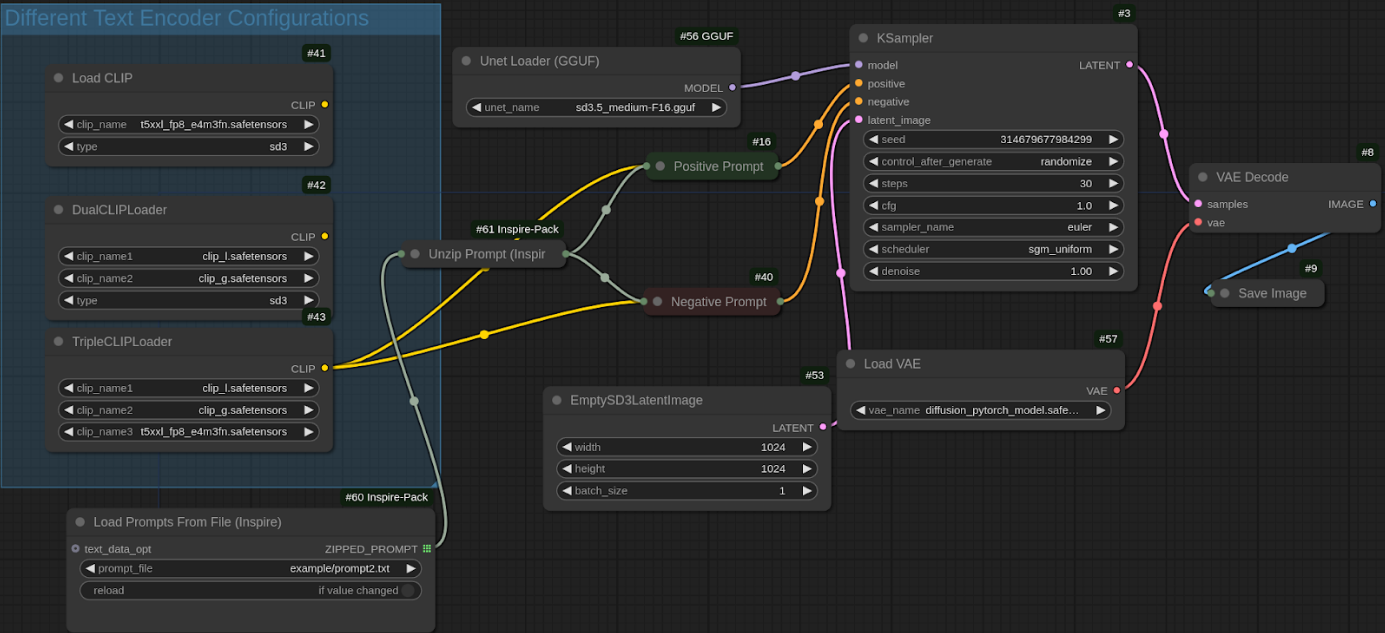
\includegraphics[width=1\linewidth]{ComfyUI-workflow}
	\caption{Representation of the ComfyUI workflow for SD3.5 image generation pipeline. The connections between the different nodes are marked by colored lines. The inference parameter details are shown in the KSampler node.}
	\label{fig:comfyui-workflow}
\end{figure}

Another custom node \texttt{Inspire Pack} \cite{inspirepack} was utilized in this project to make one-click generation of images from a text file containing multiple prompts possible. This custom node reads all the prompts in a zipped fashion from the text file and then unzips them and feeds them into the \texttt{Positive Prompt} and \texttt{Negative Prompt} nodes. 

This pipeline was used to generate a set of 100 images for each model from the generated text prompts as discussed in the next section. The average inference time of each image for FLUX.1-dev, SD3, SD3.5 was 12 minutes, 4 minutes, and 6 minutes respectively.

\subsection{Evaluation Metrics Methodology}
We downloaded 100 image caption pairs from \texttt{Conceptual Captions}, a Google Research Dataset. 
The captions provided along with the images were not descriptive enough to generate images 
using the diffusion models. An advanced vision model Microsoft \texttt{florence-2} integration was used on Hugging Face 
to generate more descriptive captions for the downloaded images. These prompts were used for text to image generation 
in the three selected models. This section describes the methodology used to evaluate the selected diffusion models. 

\subsubsection{Inception Score}
The Inception Score (IS) evaluates the quality and diversity of generated images. A pre-trained Inception V3 model was used with 
\texttt{InceptionScore} from torchmetrics. The images were resized to 299 x 299 for compatability and then converted to tensors. The Inception Score
and Standard Deviation was then calculated for the set of generated images of each diffusion model. The mean IS and SD were used for our comparison and analysis.

\subsubsection{CLIP score}
The CLIP score measures how well the generated images align with their textual prompts. The generated images were 
preprocessed into tensors and all the captions of the generated images were stored in a text file. These were the inputs to \texttt{CLIPScore} from 
torchmetrics, a pre-trained CLIP model(openai/clip-vit-base-patch16) which was 
used to compute the similarity scores between them. The CLIP score of a model was taken as the mean of CLIP scores 
of the 100 generated images of the model. 

\subsubsection{Fréchet Inception Distance}
FID calculates the similarity between the distributions of real and generated images 
in feature space. It captures both the quality and realism of generated images. The real and their corresponding generated images 
were given as inputs to the \texttt{FrechetInceptionDistance} function from torchmetrics.

\subsubsection{TIFA}
TIFA measures how faithfully the generated images represent their textual prompts 
by leveraging a Visual Question Answering(VQA) model. The TIFA methodology used here is similar to the one mentioned in \cite{Yushi2023}. Question answer pairs generated for each 
textual prompt using GPT-3. Since these questions were generic and not specific to the textual description, 
the set of questions and answers were created manually for the 100 images. 5 question answer pairs which asked about 
the subject, color in the image, presence of people, weather, etc were created for each textual prompt. A BLIP VQA model 
(Salesforce/blip-vqa-base) was used to the answer the questions given the generated image. A pre-trained BERT model from Hugging Face 
was used to compute the similarity between expected answers and the answers 
given by the VQA model. If the similarity score was above 0.7, it was deemed to be the right answer. 
The total number of correct answers and the total number of questions were recorded and used to calculate the 
TIFA score.

\subsection{CLIP MMD}
CLIP MMD is an integration of MMD techniques into CLIP framework and helps in quantifying text-to-image generative model performance. FID assumes normality of distributions which is often violated. Whereas MMD does not rely on such assumptions. Also, MMD is less dependent on sample size compared to FID. These characteristics makes MMD more reliable and consistent across different evaluation settings. Studies also show that CLIP MMD aligns better with human judgments than FID, particularly in cases involving progressive distortions or subtle improvements in image quality. To measure the CLIP MMD score for the chosen models, same image pairs used for TIFA evaluation was used as CLIP MMD measures the distance between real and generated images. A python script with Embeddings from the \verb|clip_mmd| libraries were used to calculate the score for each model.   

\section{Results and Analysis}
Table 2 captures the results from metrics evaluation. 
\begin{table}[H]
	\centering
	\begin{tabular}{p{2in} p{0.5in} p{0.5in} p{0.5in} p{0.5in} p{0.8in}}
		\toprule
		\textbf{Model} & \textbf{IS} & \textbf{CLIP} & \textbf{FID} & \textbf{TIFA} & \textbf{CLIP MMD}\\
		\midrule
		Stable Diffusion 3 Medium & 6.413 & 18.847 & 180.193 & 0.838 & 0.548\\
		Stable Diffusion 3.5 Medium & 6.127 & 18.744 & 183.266 & 0.824 & 0.497\\
		FLUX.1-dev & 6.247 & 18.805 & 181.133 & 0.917 & 0.438\\
		\bottomrule
		\\
	\end{tabular}
	\label{tab:metrics}
	\caption{Evaluated comparison metrics}
\end{table}

From this data it can be inferred that for the used setup, Stable Diffusion 3 Medium shows high IS, CLIP and FID scores. Whereas FLUX.1-dev has better numbers in terms of TIFA and CLIP MMD scores among the models compared. FLUX.1-dev demonstrates excellent semantic alignment and fidelity to text prompts. The lowest CLIP MMD shows strong multi modal alignment FLUX.1-dev model holds. Stable Diffusion 3 Medium has slightly better FID than FLUX.1-dev, suggesting marginally more realistic image quality in terms of distribution similarity to real data. Stable Diffusion 3.5 Medium performs slightly worse across most metrics compared to its predecessor (Stable Diffusion 3 Medium). From this data we can conclude that Stable Diffusion 3 Medium and  FLUX.1-dev are suitable for applications such as creative content generation, diverse dataset generation for training machine learning models. Also, the high TIFA score of FLUX.1-dev makes it ideal candidate for scientific or educational illustrations where text fidelity is crucial. These scores can vary depending on the flow setup and other implementation intricacies. The table just demonstrates an overall picture from our comparative study.\par Images generated for the text prompt: "The image is a collage of three photos showing how to make 10 minute DIY leather pulls. The first photo on the top left shows a close-up of a black cabinet door with two leather handles attached to it. The handles are brown and appear to be made of leather. The second photo in the top right shows the same leather handles hanging on the door. The third photo shows a black wardrobe with a coat rack and a potted plant on the floor. The text on the image reads "10 Minute DIY Leather Pulls"." are captured in figures ~\ref{sd3},~\ref{sd3.5}, and ~\ref{flux}. The images illustrates the difference in images generated using the models compared to an good extent. We can see that the image generated using FLUX.1-dev (Fig~\ref{flux}) is realistic and it was able to embed the text accurately in the image.

\begin{figure}[H]
	\centering
	\begin{minipage}{0.3\textwidth}
		\centering
		
\includegraphics[width=\textwidth]{sd3leather.png}
		\caption{SD3 Medium}
		\label{sd3}
	\end{minipage}
	\hfill
	\begin{minipage}{0.3\textwidth}
		\centering
		
\includegraphics[width=\textwidth]{sd3.5leather.png}
		\caption{SD3.5 Medium}
		\label{sd3.5}
	\end{minipage}
	\hfill
	\begin{minipage}{0.3\textwidth}
		\centering
		
\includegraphics[width=\textwidth]{fluxleather.png}
		\caption{FLUX.1-dev}
		\label{flux}
	\end{minipage}
\end{figure}



% \section{Workload Distribution}

% \subsection{Model Setup and Implementation (Vaibhav Sharan, Ansh Sharma)}
% \begin{itemize}
%     \item Set up local environments for Stable Diffusion, FLUX.1, and Kwai-Kolors
%     \item Implement image generation scripts for each model
% \end{itemize}

% \subsection{Quantitative Metrics Implementation (Krishnaprasad Palamattam Aji)}
% \begin{itemize}
%     \item Developed scripts for IS, FID, CLIP Score and TIFA calculation for all 3 models
% \end{itemize}

% \subsection{Data Collection and Processing (Unnikrishnan Madhavan)}
% \begin{itemize}
%     \item Create diverse text prompts dataset
%     \item Develop scripts for TIFA metrics
% \end{itemize}

% \subsection{Analysis and Report Writing (All Team Members)}
% \begin{itemize}
%     \item Analyze results and compare model performances
%     \item Write findings and prepare visualizations
% \end{itemize}
\section{Team Member Contribution}
\textbf{Vaibhav Sharan}
\begin{itemize}
    \item Performed the model selection process
    \item Implemented the image generation pipeline
    \item Generated images from the text prompts for all the diffusion models 
\end{itemize}
\textbf{Krishnaprasad Palamattam Aji}
\begin{itemize}
    \item Prepared descriptive textual inputs for image generation in all 3 models
    \item Script generation for calculating IS, FID, CLIP Score and TIFA score of all the models
\end{itemize}
\textbf{Unnikrishnan Madhavan}
\begin{itemize}
	\item Setup the script and environment for CLIP MMD Calculation
	\item Analyzed the results and performed a thorough study to understand the different use cases of each models and their trade offs
\end{itemize}
\textbf{Ansh Sharma}
\begin{itemize}
    \item Collaborated with team members to interpret the results of each metric and identify trends or patterns in model performance.    
    \item Assisted in preparing slides or visual representations of the data and findings for project presentations.
\end{itemize}


\section{Future Scope}
This study opens up several avenues for future research:
\begin{itemize}
    \item \textbf{Examining New Models:} Future studies can look at multimodal models and newer versions of Stable Diffusion (like SD 4.0) for more dynamic image production.
    \item \textbf{Domain-certain Fine-Tuning:} By optimizing models for specialized domains such as fashion design or medical imaging, results for certain industries can be improved.
    \item \textbf{Advanced Evaluation Criteria:} It might be feasible to better capture aspects of created images including texture, semantic accuracy, and originality by developing more intricate criteria.
    \item \textbf{Model Optimization:} These models are made more usable for real-time applications by reducing computation costs through techniques like knowledge distillation and pruning.
    \item \textbf{Ethical and Bias Considerations:} Future studies should address model biases and fairness to guarantee ethical use in text-to-image generation.
\end{itemize}

\section{Challenges Faced}
We ran into a number of issues during the research that hindered our ability to compare diffusion models in a consistent and seamless manner:

\begin{itemize}
    \item \textbf{Problems with Model Configuration:} The study first employed the FLUX.1-dev, Kolors, and SD3. Later, we switched to SD3.5 Medium instead of Kolors, which created more overhead in terms of model configuration and implementation and to guarantee consistent input-output compatibility.
    
    \item \textbf{Performance Variability:} Direct comparisons were challenging due to the models’ performance variability in areas like image quality, text-to-image alignment, and variety.
    
    \item \textbf{Data and Prompt Generation:} In order to improve the descriptiveness of the Conceptual Captions dataset, sophisticated models such as Microsoft Florence-2 were employed, which increased processing complexity and time.
    
    \item \textbf{Computational Constraints:} The increased complexity of newer models led to longer inference times, and even with quantized versions, the inference time remained a bottleneck for generating large sets of images.
    
    \item \textbf{Limitations of Open-Source Models:} The study was limited to open-source models, which, while accessible, lacked certain proprietary optimizations and features that could have improved performance and customization.
\end{itemize}

\section{Conclusion}
In this study, we conducted a comprehensive comparison of diffusion models for text-to-image generation, focusing on their performance across multiple metrics, including IS, CLIP, FID, TIFA, and CLIP MMD. We implemented a image generation pipeline of the selected models. These pipelines were fed by text prompts generated by the methods discussed to create the set of images for our metrics calculations. The results revealed distinct strengths and weaknesses among the models, providing valuable insights into their suitability for various applications. All the three models generate images with decent diversity and quality. Notably, FLUX.1-dev demonstrated superior text-image alignment, fidelity, and text embedding capabilities, as evidenced by its TIFA and CLIP MMD scores. 

\newpage

%Bibliography
\bibliographystyle{unsrt}  
\bibliography{references}  


\end{document}
